\documentclass[11pt,a4paper]{article}
\usepackage[T1]{fontenc}
\usepackage[utf8]{inputenc}
\usepackage[margin=1in]{geometry}
\usepackage{amsmath,amssymb,amsthm}
\usepackage{stmaryrd}
\usepackage{booktabs}
\usepackage{tabularx}
\usepackage{array}
\usepackage{enumitem}
\usepackage{listings}
\usepackage{xcolor}
\usepackage[expansion=false]{microtype}
\usepackage{tikz}
\usetikzlibrary{arrows.meta,positioning,fit,calc}
\usepackage[htt]{hyphenat}
\usepackage[hidelinks,pdftitle={F1R3Comb-Mat: the rho combinators as sparse linear algebra, in Rust}]{hyperref}
\setlength{\emergencystretch}{3em}

\newcommand{\code}[1]{\texttt{#1}}
\newcommand{\Comb}{\textsc{F1R3Comb}}
\newcommand{\Mat}{\textsc{F1R3Comb-Mat}}
\newcommand{\Kind}{\textsc{K1ndl1ng}}
\newcommand{\Camp}{\textsc{CampF1R3}}
\newcommand{\Bell}{\textsc{B3ll0ws}}
\newcommand{\Fx}{\textsc{F1R3x}}
\newcommand{\Rhobots}{\textsc{Rhobots}}
\newcommand{\MUST}{\textsc{must}}
\newcommand{\MUSTNOT}{\textsc{must not}}
\newcommand{\SHOULD}{\textsc{should}}
\newcommand{\SHOULDNOT}{\textsc{should not}}
\newcommand{\MAY}{\textsc{may}}

\newcommand{\quo}[1]{@#1}
\newcommand{\drp}[1]{{*}#1}
\newcommand{\nil}{\mathbf{0}}
\newcommand{\nequiv}{\equiv_{\mathcal{N}}}
\newcommand{\nms}[1]{\mathcal{N}^{*}(#1)}
\newcommand{\Nsort}{\mathsf{N}}
\newcommand{\Psort}{\mathsf{P}}
\newcommand{\red}{\longrightarrow}
\newcommand{\wred}{\longrightarrow^{*}}
\newcommand{\scong}{\equiv}
\newcommand{\comps}[1]{\lvert #1 \rvert}

\newcommand{\mm}{\mathsf{m}}
\newcommand{\dd}{\mathsf{d}}
\newcommand{\kk}{\mathsf{k}}
\newcommand{\fw}{\mathsf{fw}}
\newcommand{\bl}{\mathsf{b}_{\mathsf{l}}}
\newcommand{\br}{\mathsf{b}_{\mathsf{r}}}
\newcommand{\sy}{\mathsf{s}}
\newcommand{\ev}{\mathsf{e}}
\newcommand{\qq}{\mathsf{q}}
\newcommand{\cons}{\mathsf{cons}}
\newcommand{\consm}{\mathsf{cons}_{\mm}}
\newcommand{\consd}{\mathsf{cons}_{\dd}}
\newcommand{\conss}{\mathsf{cons}_{\sy}}
\newcommand{\conse}{\mathsf{cons}_{\ev}}
\newcommand{\consf}{\mathsf{cons}_{\fw}}

\newcommand{\Spec}{\mathcal{S}}
\newcommand{\Nm}{\mathcal{N}}
\newcommand{\cre}[1]{a^{\dagger}_{#1}}
\newcommand{\ann}[1]{a_{#1}}
\newcommand{\Wt}{\mathsf{W}}

\theoremstyle{definition}
\newtheorem{definition}{Definition}[section]
\newtheorem{requirement}[definition]{Requirement}
\newtheorem{decision}[definition]{Decision}
\newtheorem{obligation}[definition]{Obligation}
\newtheorem{hazard}[definition]{Hazard}
\newtheorem{erratum}[definition]{Erratum}
\newtheorem{remark}[definition]{Remark}
\newtheorem{example}[definition]{Example}
\theoremstyle{plain}
\newtheorem{proposition}[definition]{Proposition}
\newtheorem{lemma}[definition]{Lemma}

\lstset{
  basicstyle=\ttfamily\footnotesize,
  columns=fullflexible,
  keepspaces=true,
  breaklines=true,
  frame=leftline,
  framesep=6pt,
  xleftmargin=8pt,
  rulecolor=\color{black!30},
  showstringspaces=false,
}

\title{\textbf{\Mat}\\[1mm]
\large The rho combinators as sparse linear algebra:\\
a Rust implementation of the matrix representation,\\
the bulk-synchronous machine, and the transfer operator\\[2mm]
\normalsize Specification v0.1 --- companion to \Comb{} v0.2}
\author{F1R3FLY.io}
\date{22 September 2026}

\begin{document}
\maketitle

\begin{abstract}
\noindent
\emph{Rho combinators as sparse linear algebra} \cite{matnote} shows that a
combinator state is an occupation vector, that the one-step relation is a sum
of ladder-operator monomials, and --- the practical finding --- that the matrix
worth multiplying is not the transition matrix of the reduction graph but the
incidence of atom occurrences against names, which is term-sized. Redex
finding is a join on that incidence, conflict detection is a second sparse
product, and a machine step fires a maximal independent set of redexes, so
machine steps count causal depth. A Python reference
(\code{rhocombmat.py}, \code{experiments.py}) validates the join against naive
enumeration and measures width on four term families. \Comb{} v0.2
\cite{combspec} specifies the compiler from kernel rho to the combinators and
an interleaving machine built on \Camp. Nothing takes a combinator term to its
matrix representation in Rust, and nothing runs it there.

This document specifies that arrow and what sits on it: three crates in the
\code{campf1r3} workspace that intern a \Comb{} term into a fixed-width,
integer-indexed representation; find redexes by joins derived from one shared
rule table; select a maximal independent set by a bit-exactly specified
priority function; fire it; and, on the destructor-free sublattice, materialise
the transfer operator over reachable markings and close it. The design keeps
every invariant \Comb{} v0.2 established --- presentation~A, the
$\mm$/$\qq$ sort asymmetry, canonical encodings, no external dependencies,
bit-identical results across core counts and WebAssembly --- and reconciles the
one place the two documents appear to disagree, the payload of $\qq$
(Decision~\ref{dec:qrow}).

Checking the note against its own reference turned up three errors that the
implementation cannot inherit, because it asserts the invariants in question.
The atom-count lemma of draft~3 \cite[Lem.~9.2]{draft3} is false for $\bl$,
$\br$ and $\sy$, so the length bound of \cite[Prop.~9.9]{draft3} and the
nilpotency index of \cite[Thm.~6.1(ii)]{matnote} are wrong, though both
conclusions survive under a weighted grading (Erratum~\ref{err:atomcount}).
The message-count invariant of \cite[Thm.~6.1(iii)]{matnote} is broken by the
$\mathsf{quote}$ rule and holds for messages plus stores
(Erratum~\ref{err:msgcount}). And the reference enumerates symmetric
constructor matches twice, which is harmless to the step and wrong for the
mass-action coefficient (Erratum~\ref{err:symmetric}).
Section~\ref{sec:paper} lists these with proposed amendments. Key words
\MUST, \MUSTNOT, \SHOULD, \MAY{} are used in the sense of RFC~2119.
\end{abstract}

\tableofcontents

%======================================================================
\section{Purpose and scope}\label{sec:purpose}

\subsection{The gap}

\cite{matnote} is a design analysis with a correctness reference. Its six
claims (C1)--(C6) are about a representation and a step discipline; its
reference implementation is explicitly ``a correctness reference, not a
performance artefact''; and its development plan (\S11, phases P0--P6) puts the
Rust port at P3, after a width measurement (P2) that needs the compiler. The
compiler now has a specification \cite{combspec}. This document is P0, P3 and
P6 of \cite{matnote}, specified against \Comb{}'s term type, and it supplies
the instrument P2 needs.

Two properties the Python reference is entitled to leave loose are properties
this implementation is not. The reference assigns name indices and occurrence
identities by insertion into Python dictionaries, and chooses the independent
set by a shuffled order; its runs are reproducible only by seed and only in
one process. \Comb{} v0.2 requires the compiled term, its hash, the event
stream and the final scene to be bit-identical across runs, hosts, core counts
and WebAssembly (\cite[Req.~12.4]{combspec}). A second machine over the same
terms that cannot meet that requirement cannot be differentially tested
against the first, and cannot be ported to a device with the exit criterion
\cite[P4]{matnote} sets --- identical step traces under a fixed seed.

\subsection{What exists today}

\begin{center}
\begin{tabularx}{\linewidth}{@{}l>{\raggedright\arraybackslash}X@{}}
\toprule
Artefact & What it gives this project\\
\midrule
\code{rho-combinators/rhocomb-matrix} & The state space (\S4), the transfer
operator and its three rule classes (\S5), the lattice-as-finiteness theorem
(Thm.~6.1), the incidence matrix and the join table (\S7), the step and its
soundness (\S8), reflection as an intern table (\S9), measurements (\S10), the
plan and obligations (\S11, \S13)\\
\code{rho-combinators/rhocombmat.py} & The reference machine: intern table,
occurrence store, incidence, joins, conflict product, greedy independent set,
firing\\
\code{rho-combinators/experiments.py}, \code{results.txt} & Four term
families E1--E4 and a 400-state validation; every number in
\cite[\S10]{matnote}\\
\code{rho-combinators/f1r3comb-spec-v02} & The target term type
(\code{f1r3comb-term}), presentation~A, the encoding, the tag table, the rule
table requirement, the \Camp{} machine, the diagnostics and portability
envelope this document inherits\\
\code{rho-combinators/rho-combinators-draft3} & The calculus
(Def.~3.3), the lattice invariants (\S9), the shortcuts (Rem.~6.7)\\
\code{rho-combinators/rhocomb-logic} & Components as a complete invariant
(Def.~2.9), drop elimination (Lem.~2.8), injective quotation (Prop.~2.10),
occupancy (Thm.~6.5); the eventual consumer of the operator layer\\
\code{campf1r3} (the repository) & The workspace: \code{k1ndl1ng-norm}'s
\code{Hash32} and \code{blake2b\_256}, \code{campf1r3-core}, \code{f1r3x};
no external dependencies\\
\bottomrule
\end{tabularx}
\end{center}

\subsection{Nomenclature}\label{sec:nomen}

\begin{center}
\begin{tabularx}{\linewidth}{@{}l>{\raggedright\arraybackslash}X@{}}
\toprule
Term & Meaning in this document\\
\midrule
\emph{term} & A \code{f1r3comb\_term::Term}: a drop-free normal form under
presentation~A, a flat multiset of atoms \cite[Req.~4.4]{combspec}\\
\emph{name id} & A \code{NameId(u32)}: the in-run index of a name modulo
$\nequiv$\\
\emph{row} & One atom occurrence in the machine: a shape and a fixed-width
tuple of name ids\\
\emph{row ref} & \code{(Shape, u32)}: a row's position in its shape table;
the machine-level occurrence identity of \cite[Def.~8.1]{matnote}\\
\emph{incidence} & The family $M^{A}_{j}$ of \cite[Def.~7.1]{matnote}; here
implicit in the shape tables\\
\emph{species} & A shape with a tuple of name ids \cite[Def.~4.1]{matnote}; a
row's value, forgetting its position\\
\emph{marking} & A finite multiset of species; a basis vector
$|\gamma\rangle$ of the state space\\
\emph{redex} & A rule together with the row refs it consumes, in premise
order\\
\emph{step} & The firing of one independent set of redexes\\
\emph{width} & The size of a step\\
\emph{grading} & The function $\Wt$ of Erratum~\ref{err:atomcount}\\
\bottomrule
\end{tabularx}
\end{center}

\noindent
The product name is \Mat{}, written \code{f1r3comb-mat}, \code{f1r3comb-par}
and \code{f1r3comb-op} in crate names and \code{comb-mat}, \code{comb-width}
and \code{comb-op} in \Fx{} subcommands. The name is provisional and \MAY{} be
changed before M0 without affecting any requirement.

\subsection{Goals}

\begin{enumerate}[leftmargin=1.6em]
\item A total, lossless, round-trippable map from \Comb{} terms to the matrix
representation of \cite[\S7]{matnote}, and back.
\item Redex finding as joins on the incidence, derived mechanically from the
rule table \Comb{} already requires \cite[Req.~4.7]{combspec}, with three
independent finders that \MUST{} agree.
\item A bulk-synchronous machine whose step is a maximal independent set,
defined bit-exactly, so that the host sequential, host threaded and any
future device backend produce identical traces.
\item Instrumentation sufficient to run the width measurement that gates
device work \cite[Obl.~13.7]{matnote}.
\item On the destructor-free sublattice, the transfer operator over reachable
markings, its triangular structure, its closure, and the pre-image primitive
the logic's modality needs \cite[Rem.~11.1]{matnote}.
\item The \Comb{} portability envelope: no external dependencies,
\code{forbid(unsafe\_code)}, \code{wasm32-unknown-unknown}-clean,
bit-identical across hosts and core counts.
\end{enumerate}

\subsection{Non-goals}\label{sec:nongoals}

\begin{enumerate}[leftmargin=1.6em]
\item \textbf{Device code.} No GPU kernel is specified for the workspace.
Section~\ref{sec:device} specifies the backend contract a device
implementation \MUST{} meet and places it outside the workspace, because
every device API is an external dependency. It is gated on
Obligation~\ref{obl:width}.
\item \textbf{Presentation B.} The matrix representation is A-only; this is
forced, not chosen (\cite[Rem.~3.1]{matnote}; Decision~\ref{dec:aonly}).
\item \textbf{Weights.} Boolean and natural-number semirings only. The
\code{Semiring} trait of Section~\ref{sec:sparse} is the seam where the
weighted readings attach, and nothing here depends on them.
\item \textbf{The logic.} The operator layer exposes $T$, its closure and
$T^{\top}\chi$. It \MUSTNOT{} implement satisfaction, characteristic formulae
or model checking, which are \cite{logic}'s.
\item \textbf{The history unfolding.} Triangularity with $\ev$ present via
the universal cover \cite[\S6.1, route (1)]{matnote} is deferred.
\item \textbf{Garbage collection of the intern table.} Deferred
(\cite[Obl.~13.3]{matnote}; Requirement~\ref{req:reports}); inert rows are counted, not collected.
\end{enumerate}

%======================================================================
\section{Position relative to \Comb}\label{sec:position}

\subsection{Two machines, one term type}

\Comb{} v0.2 runs a term by instantiating \Camp: an interleaving machine, one
comm per event, races resolved by the store's order key
\cite[Dec.~8.1]{combspec}. \Mat{} runs the same term by maximal progress:
every step fires a maximal set of pairwise disjoint redexes. The two are
different resolvers for the same nondeterminism \cite[Rem.~8.5]{matnote}, and
neither is a refinement of the other. What they share is fixed here.

\begin{center}
\begin{tabularx}{\linewidth}{@{}l>{\raggedright\arraybackslash}X>{\raggedright\arraybackslash}X@{}}
\toprule
& \Comb{} machine (\code{f1r3comb-run}) & \Mat{} (\code{f1r3comb-par})\\
\midrule
Input & \code{Term} & \code{Term}\\
State & \Camp{} store keyed by \code{Hash32} & shape tables of
\code{NameId} rows\\
Name identity & content hash of the encoding & in-run structural intern,
content hash at the boundary\\
Event & one comm & one step, a maximal independent set\\
Resolver & store order key & priority function of
Definition~\ref{def:prio}\\
Rule source & the shared rule table & the shared rule table\\
Output & a scene (\code{Term}) & a scene (\code{Term})\\
\bottomrule
\end{tabularx}
\end{center}

\subsection{Decisions inherited and decisions taken}

\begin{decision}[Presentation A only]\label{dec:aonly}
\Mat{} implements presentation~A. With \Comb's \code{presentation-b} feature
enabled, the three crates \MUST{} compile to stubs whose entry points return
\code{comb-mat-presentation}, so that a workspace-wide feature unification
does not break the build. Under B a message payload is a process, rows are
ragged, and requirement (G1) of \cite[\S2.1]{matnote} fails by construction.
\end{decision}

\begin{decision}[A store row holds the quotation of its payload]
\label{dec:qrow}
In the term type, $\qq(a,p)$ carries a process, and \Comb{}'s reversal of
v0.1 on this point \cite[Dec.~4.9, Rem.~4.10]{combspec} stands. In the
matrix representation, the row for $\qq(a,p)$ is $(\qq,\ \mathrm{id}(a),\
\mathrm{id}(\quo{p}))$. The two statements do not conflict, and this decision
records why:
\begin{enumerate}[leftmargin=1.6em]
\item the row is a \emph{representation}, not a sort: under A, $\quo{-}$ is
injective on drop-free normal forms \cite[Prop.~2.10]{logic}, so storing
$\mathrm{id}(\quo{p})$ loses nothing and export recovers $p$ exactly;
\item the $\mm$/$\qq$ distinction the logic turns on \cite[Rem.~2.5]{logic} is
carried by the \emph{shape tag}, which is preserved; a $\qq$ row and an $\mm$
row with equal id tuples are different species;
\item the matrix representation is not a term type, and
\MUSTNOT{} be offered to the logic tooling as one
(Requirement~\ref{req:notaterm}).
\end{enumerate}
The effect is the one \cite[Rem.~3.1]{matnote} wants: every row is a
fixed-width tuple of integers, and the $\mathsf{quote}$ rule is a field copy
(rule class (a)).
\end{decision}

\begin{decision}[Decode by arena read]\label{dec:decode}
\cite[Req.~8.3]{combspec} forbids the \Comb{} machine to realise
$\mathsf{eval}$ by projecting the payload out of the name, because the
short-circuit is unsound under B. \Mat{} realises it exactly so --- a read of
the intern arena at $v$ --- and is entitled to, because it is A-only
(Decision~\ref{dec:aonly}) and because interning applies drop elimination
before any component is stored (Requirement~\ref{req:internnorm}). The crate
\MUST{} carry a test asserting, for every name in a corpus, that the arena
entry equals the atom multiset of the smart-constructed $\drp{v}$ in
\code{f1r3comb-term}.
\end{decision}

\begin{decision}[One rule table]\label{dec:ruletable}
The rule table \cite[Req.~4.7]{combspec} \MUST{} live in \code{f1r3comb-term}
(module \code{rules}), not in \code{f1r3comb-run}, and both machines \MUST{}
be dispatches over it. Joins, conclusions, rule classes and the grading of
Erratum~\ref{err:atomcount} are all derived from the table; no rule is
special-cased in \Mat's control flow. This is a request of \Comb{}
(Section~\ref{sec:paper}, item~6).
\end{decision}

\begin{decision}[Shortcuts are supported]\label{dec:shortcuts}
With \Comb's \code{shortcuts} feature, the shape set grows to fifteen. \Mat{}
\MUST{} support it through the rule table alone. Draft~3 names
$\conse$ and $\consf$ but does not state their rules
\cite[Rem.~3.10, Rem.~6.7]{draft3}; this document fixes them as the
completions consistent with \cite[Req.~7.12]{combspec}'s arities:
\[
\conse(a,f) \mid \mm(a,u) \red \mm(f,\quo{\ev(u)}),
\qquad
\consf(a,b,f) \mid \mm(a,u) \mid \mm(b,v) \red \mm(f,\quo{\fw(u,v)}).
\]
Section~\ref{sec:paper} asks draft~3 to state them.
\end{decision}

%======================================================================
\section{The representation}\label{sec:rep}

\subsection{Names and the intern table}

\cite[Def.~4.3]{matnote} realises $\Nm$ as a bijection between integers and
canonical component multisets. The Rust type is:

\begin{lstlisting}
#[derive(Copy, Clone, PartialEq, Eq, PartialOrd, Ord, Hash, Debug)]
pub struct NameId(pub u32);

#[derive(Copy, Clone, PartialEq, Eq, PartialOrd, Ord, Hash, Debug)]
pub struct Row { pub shape: Shape, pub args: [NameId; 4] }   // unused slots = NameId::PAD

pub struct InternTable {
    arena:  Vec<Row>,                 // components of every name, contiguous
    span:   Vec<(u32, u32)>,          // NameId -> (offset, len) into arena
    key:    HashMap<Box<[Row]>, NameId>,   // structural key -> id (std only)
    depth:  Vec<u32>,                 // quotation depth, for canonical export
    chash:  Vec<Option<Hash32>>,      // content hash, computed lazily
    budget: NameBudget,
}
\end{lstlisting}

\begin{definition}[Structural key]\label{def:skey}
The key of a name is the sorted slice of its component rows, sorted by
\code{Row}'s derived order. By \cite[Def.~2.9]{logic} components are a
complete invariant, and by induction on quotation depth two names receive the
same id iff they are $\nequiv$ (\cite[Prop.~2.10]{logic}).
\end{definition}

\begin{requirement}[The hot path is hash-free]\label{req:hashfree}
\code{quote} (insert-or-get by structural key) and \code{drop} (arena read)
\MUSTNOT{} compute BLAKE2b. The content hash of \Comb{}
\cite[Req.~4.12]{combspec} is computed only at the boundary --- export,
tracing, canonical relabelling --- memoised per id in \code{chash}. This is
\cite[Obl.~13.2]{matnote} discharged: the canonical, run-stable hash the note
asks for already exists, it is \Comb's encoding hash, and the machine does not
need it to run.
\end{requirement}

\begin{requirement}[Key and hash agree]\label{req:keyhash}
For all ids $i,j$: $i = j$ iff \code{chash(i) == chash(j)}, modulo BLAKE2b
collision. A property test \MUST{} assert this on every corpus run, and the
debug build \MUST{} assert it whenever two ids' hashes are both materialised.
A collision is a \code{comb-mat-hash-collision} diagnostic, never a merge.
\end{requirement}

\begin{requirement}[Interning normalises]\label{req:internnorm}
Components entering the arena \MUST{} be drop-free, which import guarantees
because \code{Term} is (\cite[Req.~4.4]{combspec}), and constructor firing
guarantees because every class (b) conclusion is built from rows. The
$\cons$ rule's union $\mathrm{drop}(u) \uplus \mathrm{drop}(r)$ \MUST{} be
computed as a multiset merge of two sorted arena spans, so the result is its
own key without a further sort.
\end{requirement}

\begin{remark}[Interning order is a gauge freedom, and is fixed anyway]
\cite[Rem.~4.4]{matnote} observes that ids depend on insertion order and that
nothing observable may depend on them. That remains true of the semantics.
But Requirement~\ref{req:det} needs the machine's internal choices to be
reproducible, and those choices read row positions and ids. \Mat{} therefore
fixes insertion order (Requirement~\ref{req:insertorder}) so that ids are
reproducible, and separately forbids ids from crossing any external boundary
(Requirement~\ref{req:noidleak}). The gauge is fixed for determinism and
hidden for semantics.
\end{remark}

\begin{requirement}[Ids never leave the process]\label{req:noidleak}
No trace event, report, diagnostic, export or public API return value
\MAY{} contain a \code{NameId} or a row position, except the \code{.cmat}
format of Section~\ref{sec:cmat}, which uses canonically relabelled ids.
Externally a name is its \code{Hash32}.
\end{requirement}

\begin{requirement}[Budget]\label{req:budget}
\cite[Req.~8.8]{combspec}'s budget carries over: maximum distinct names,
maximum components per name, maximum arena length. Exceeding any \MUST{} halt
the step before it commits, with \code{comb-name-budget} naming the rule and
the redex's consumer as a content hash.
\end{requirement}

\subsection{State: shape tables}

\begin{definition}[State]\label{def:state}
A state is one table per enabled shape. The table for shape $A$ of arity $k$
is $k$ columns of \code{NameId}, all of equal length; row $i$ of the table is
the $i$-th occurrence of $A$.
\end{definition}

\begin{lstlisting}
pub struct ShapeTable { pub cols: [Vec<NameId>; 4], pub len: u32 }  // cols[j] unused for j >= arity
pub struct State { pub tables: [ShapeTable; SHAPES] }                 // SHAPES = 13, or 15 with shortcuts
\end{lstlisting}

\begin{requirement}[Structure of arrays]\label{req:soa}
Columns \MUST{} be separate contiguous arrays. This is (G1) of
\cite[\S2.1]{matnote} and it is what makes the incidence implicit
(Definition~\ref{def:inc}). An array of \code{Row} structs \MUSTNOT{} be used
for the state; it is used only for the arena, where rows of mixed shape
must be contiguous for decode.
\end{requirement}

\begin{definition}[Incidence, implicit]\label{def:inc}
The Boolean matrix $M^{A}_{j}$ of \cite[Def.~7.1]{matnote} has exactly one
nonzero per row, at column \code{tables[A].cols[j][i]}. Its CSR form is
therefore \code{indptr} $= 0,1,\dots,n$ and \code{indices}
$=$ \code{cols[j]}. The column array \emph{is} the matrix. It \MUSTNOT{} be
materialised separately in the production path; the generic finder of
Section~\ref{sec:finders} \MAY{} materialise it, through the
\code{Csr::from\_column} view, for validation.
\end{definition}

\subsection{Import and export}

\begin{requirement}[Import]\label{req:import}
\code{State::import(\&Term, \&mut InternTable)} \MUST{} flatten the term's
components in encoding order and push one row per atom, interning every name
argument bottom-up with an explicit stack --- the workspace's no-recursion
rule \cite[Req.~7.1]{combspec} applies. An import memo keyed by
\code{Hash32} \MAY{} be used to skip re-interning a name already seen; it
\MUST{} agree with the structural key (Requirement~\ref{req:keyhash}). The
payload of $\qq$ is interned as its quotation (Decision~\ref{dec:qrow}).
\end{requirement}

\begin{requirement}[Export]\label{req:export}
\code{State::export(\&InternTable) -> Term} \MUST{} rebuild the term through
\code{f1r3comb-term}'s smart constructors, rendering a $\qq$ row's second
argument by \code{drop}. Import followed by export \MUST{} be the identity on
encodings, and export followed by import \MUST{} be the identity on markings.
Both are property tests.
\end{requirement}

\begin{requirement}[Not a term type]\label{req:notaterm}
\code{State}, \code{Row} and \code{InternTable} \MUST{} be documented as a
machine representation. \cite[Req.~9.2]{combspec}'s public API for the logic
is \code{f1r3comb-term}'s, and \Mat{} \MUSTNOT{} expose a second one.
\end{requirement}

\subsection{The canonical export format}\label{sec:cmat}

A term's matrix representation is worth a file of its own, for three
consumers: a device backend in another process, the Python reference, and
golden tests. In-run ids are not canonical, so the file relabels them.

\begin{definition}[Canonical relabelling]\label{def:relabel}
Order the names reachable from a state by quotation depth, ties broken by
content hash, and assign ids $0,1,\dots$ in that order; every name's
components then refer only to smaller ids. Within each shape table, order rows
lexicographically by relabelled id tuple.
\end{definition}

\begin{requirement}[\code{.cmat}]\label{req:cmat}
The \code{.cmat} encoding \MUST{} be: a header (magic \code{CMAT}, format
version, presentation, \code{shortcuts} flag, shape count); the name table in
relabelled order, each entry a LEB128 component count followed by rows, each
row a shape tag from \cite[\S4.5]{combspec} and LEB128 ids; then the
state, per shape a LEB128 row count followed by columns. It \MUST{} satisfy:
for terms $P \scong Q$ the \code{.cmat} encodings are byte-equal. With
\Comb's canonicity theorem \cite[Obl.~5.8]{combspec} this makes the file a
function of the source congruence class.
\end{requirement}

\begin{requirement}[Python interoperability]\label{req:pyinterop}
\code{f1r3comb-check} \MUST{} ship a loader for \code{.cmat} in the Python
reference's representation (a \code{NameTable} and a \code{State}), as a
script outside the Rust build, so that Obligation~\ref{obl:pyparity} can run
the Rust and Python machines on one input.
\end{requirement}

%======================================================================
\section{The rule table, as \Mat{} reads it}\label{sec:rules}

\subsection{The table}

\begin{lstlisting}
pub enum Var { Slot(u8), Payload(u8) }           // consumer's arg j; premise j's payload
pub enum Premise { Loud { subject: u8 }, AnyAt { subject: u8 } }  // AnyAt: m or q (fw only)
pub enum Conclusion {
    Atoms(&'static [(Shape, &'static [Var])]),   // class (a)
    Encode { deliver: Var, node: NodeTemplate }, // class (b): m(deliver, @node)
    Decode { payload: Var },                     // class (c): *payload
}
pub enum NodeTemplate { Union(Var, Var), Atom(Shape, &'static [Var]) }
pub struct RuleSpec {
    pub name: &'static str, pub consumer: Shape,
    pub premises: &'static [Premise], pub conclusion: Conclusion, pub class: RuleClass,
}
\end{lstlisting}

\noindent
The rows, for the thirteen-shape calculus of \cite[Def.~3.3]{draft3} and
\cite[Def.~4.6]{combspec}:

\begin{center}\small
\begin{tabular}{@{}llll@{}}
\toprule
Rule & Consumer & Premises & Conclusion\\
\midrule
$\mathsf{dist}$ & $\dd(a,b,c)$ & loud at $a$ & $\mm(b,v_{0}) \mid \mm(c,v_{0})$\\
$\mathsf{kill}$ & $\kk(a)$ & loud at $a$ & $\nil$\\
$\mathsf{forward}$ & $\fw(a,b)$ & loud at $a$ & $\mm(b,v_{0})$\\
$\mathsf{bind_l}$ & $\bl(a,b)$ & loud at $a$ & $\fw(v_{0},b)$\\
$\mathsf{bind_r}$ & $\br(a,b)$ & loud at $a$ & $\fw(b,v_{0})$\\
$\mathsf{synch}$ & $\sy(a,b,c)$ & loud at $a$ & $\fw(b,c)$\\
$\mathsf{eval}$ & $\ev(a)$ & loud at $a$ & decode $v_{0}$\\
$\mathsf{quote}$ & $\fw(a,b)$ & quiet at $a$ & $\mm(b,v_{0})$\\
$\mathsf{make}_{\mid}$ & $\cons(a,b,c)$ & loud at $a$, $b$ & $\mm(c,\quo{(\drp{v_0}\mid\drp{v_1})})$\\
$\mathsf{make}_{\mm}$ & $\consm(a,b,c)$ & loud at $a$, $b$ & $\mm(c,\quo{\mm(v_0,v_1)})$\\
$\mathsf{make}_{\dd}$ & $\consd(a,b,c,f)$ & loud at $a$, $b$, $c$ & $\mm(f,\quo{\dd(v_0,v_1,v_2)})$\\
$\mathsf{make}_{\sy}$ & $\conss(a,b,c,f)$ & loud at $a$, $b$, $c$ & $\mm(f,\quo{\sy(v_0,v_1,v_2)})$\\
\midrule
$\mathsf{make}_{\ev}$ & $\conse(a,f)$ & loud at $a$ & $\mm(f,\quo{\ev(v_0)})$ \quad \code{shortcuts}\\
$\mathsf{make}_{\fw}$ & $\consf(a,b,f)$ & loud at $a$, $b$ & $\mm(f,\quo{\fw(v_0,v_1)})$ \quad \code{shortcuts}\\
\bottomrule
\end{tabular}
\end{center}

\begin{remark}[$\fw$ has two rows]
$\fw$ is the one consumer with two rules, one per datum kind. \Comb's machine
merges them into one \code{consume} with an \code{accepts\_quiet} pattern
\cite[\S8.2]{combspec}; \Mat{} keeps them as two rows because they join
against different tables ($\mm$ and $\qq$). The race
$\fw(a,b) \mid \mm(a,v) \mid \qq(a,p)$ \cite[Req.~8.6]{combspec} then appears
as two redexes sharing the $\fw$ row, which the conflict structure resolves.
The quiet/loud distinction therefore lives in the join, not in a matcher, and
Requirement~\ref{req:quietjoin} makes that exact.
\end{remark}

\begin{requirement}[Only a forwarder reads a store]\label{req:quietjoin}
No rule other than $\mathsf{quote}$ \MAY{} join against the $\qq$ table. A
test \MUST{} assert that for every consumer shape other than $\fw$, a state
consisting of that consumer and a $\qq$ row at its subject has no redex. This
is the inertness of an ungated gate \cite[Lem.~6.5]{draft3} in \Mat's terms.
\end{requirement}

\subsection{Rule classes}

\begin{requirement}[Class is data]\label{req:class}
Each row \MUST{} carry its class from \cite[\S5.1]{matnote}: (a) seven rules
whose conclusions are fixed multisets over premise names (including
$\mathsf{quote}$, by Decision~\ref{dec:qrow}); (b) the constructors, which
encode; (c) $\mathsf{eval}$, which decodes. A test \MUST{} assert that the
class recorded agrees with the \code{Conclusion} variant, and that exactly
one rule is class (c).
\end{requirement}

\subsection{Join plans}

\begin{definition}[Join plan]\label{def:plan}
The join plan of a rule is the list of pairs (consumer slot, premise table)
read off its premises: premise $j$ joins column $\code{subject}_{j}$ of the
consumer's table against column 0 of the $\mm$ table (loud) or of the $\qq$
table (quiet). A rule with $k$ premises has a $k$-way join, $k \le 3$.
\end{definition}

\begin{requirement}[Plans are derived]\label{req:plansderived}
Join plans \MUST{} be computed from the rule table at start-up (or
\code{const}-evaluated) and \MUSTNOT{} be written by hand. The table of
\cite[\S7.1]{matnote} is then a theorem about the derivation, and a test
\MUST{} check it: seven one-premise loud plans, one one-premise quiet plan,
two (four with \code{shortcuts}) two-premise plans, two three-premise plans.
\end{requirement}

%======================================================================
\section{Sparse algebra}\label{sec:sparse}

No external dependency is available, so the crate carries its own small
sparse layer. It is used by the generic finder, the reference conflict
product and the operator layer; the production machine uses only its
counting-sort primitive.

\begin{lstlisting}
pub trait Semiring: Copy + Eq + core::fmt::Debug {
    const ZERO: Self; const ONE: Self;
    fn add(self, o: Self) -> Self; fn mul(self, o: Self) -> Self;
}
#[derive(Copy, Clone, PartialEq, Eq, Debug)] pub struct Bool(pub bool);
#[derive(Copy, Clone, PartialEq, Eq, Debug)] pub struct Nat(pub u64);   // checked; overflow is an error

pub struct Csr<S: Semiring> { pub rows: u32, pub cols: u32,
                              pub indptr: Vec<u32>, pub indices: Vec<u32>, pub vals: Vec<S> }
impl<S: Semiring> Csr<S> {
    pub fn from_column(col: &[NameId], ncols: u32) -> Self;   // the implicit incidence view
    pub fn transpose(&self) -> Self;                          // counting sort, O(nnz + cols)
    pub fn spgemm(&self, rhs: &Self) -> Result<Self, Overflow>;  // Gustavson
    pub fn spmv(&self, x: &SparseVec<S>) -> Result<SparseVec<S>, Overflow>;
}
\end{lstlisting}

\begin{requirement}[Semantics of the layer]\label{req:sparse}
\code{spgemm} \MUST{} be Gustavson's row-by-row algorithm \cite{gustavson}
with a dense accumulator reset per row, producing sorted column indices and
no explicit zeros. \code{Nat} arithmetic \MUST{} be checked; overflow is
\code{comb-mat-overflow}, never a wrap. \code{Bool} \MAY{} store no
\code{vals} (a specialisation), provided the observable results are equal.
The layer is correct by comparison with a dense reference on random matrices
up to $64 \times 64$, as a property test.
\end{requirement}

\begin{requirement}[Bucketing primitive]\label{req:bucket}
\code{bucket(col: \&[NameId]) -> Buckets} \MUST{} return, for each name
occurring in \code{col}, the ascending list of rows carrying it, as a CSR
over the \emph{occurring} names only (sorted, deduplicated), so that its cost
is $O(n \log n)$ in the column length or $O(n)$ by radix sort, and never
proportional to the size of the intern table. It is $(M^{A}_{j})^{\top}$
restricted to its nonempty rows.
\end{requirement}

%======================================================================
\section{Redex finding}\label{sec:finders}

\subsection{The redex}

\begin{definition}[Redex]\label{def:redex}
A redex is \code{(rule: u8, consumer: u32, premises: [u32; 3])}: the rule's
index in the table, the consumer's row in its table, and for each premise the
row in the $\mm$ or $\qq$ table, padded. It is \emph{enabled} if each premise
row's subject equals the corresponding consumer slot, and the premise rows
are pairwise distinct when they are in the same table.
\end{definition}

\begin{definition}[Canonical key]\label{def:key}
The canonical key of a redex is the tuple (rule, consumer, premises) under
lexicographic order. Redex sets are always delivered sorted by canonical key.
\end{definition}

\begin{erratum}[Symmetric matches are one redex]\label{err:symmetric}
The reference enumerates ordered premise tuples subject only to distinctness
of occurrences. When two premise positions of a constructor receive
\emph{equal atoms} --- equal subject and equal payload, as in
$\cons(a,a,c) \mid \mm(a,u) \mid \mm(a,u)$ --- the two orderings consume the
same multiset and produce the same result, and the reference reports two
redexes. They are one derivation: \cite[Prop.~5.3]{matnote}'s coefficient
divides by $m_{\alpha}!$ for exactly this reason, and the reference's count is
$2$ where the proposition's is $1$. The step is unaffected (the two conflict,
and either may be chosen), and none of the E1--E4 families contain such a
match, so \code{results.txt} is unaffected. But the operator layer computes
the coefficient, and a resolver that picks one redex uniformly from the
enumerated set --- the reference's \code{run\_sequential} --- double-weights
symmetric matches, which is a semantic commitment
\cite[Obl.~13.1]{matnote} did not intend.
\end{erratum}

\begin{requirement}[Symmetry mask]\label{req:symmask}
Every finder \MUST{}, in addition to the distinctness mask of
\cite[\S7.1]{matnote}, drop an ordered premise tuple in which two positions
carrying equal atoms appear with the later position at a lower row. The
enumerated set is then in bijection with derivations, and its size is the
\code{Nat} coefficient of \cite[Prop.~5.3]{matnote} summed over results.
\end{requirement}

\subsection{Three finders}

\begin{requirement}[Three implementations, one answer]\label{req:finders}
\code{f1r3comb-par} \MUST{} provide three finders behind one trait, and
\MUST{} test that they return identical sorted redex sets on every state in
the property corpus.
\begin{enumerate}[leftmargin=1.6em]
\item \code{Naive}: for each consumer row and each rule of its shape, nested
loops over the premise tables. The oracle; no sparse code.
\item \code{Product}: per join plan, the Boolean product
$M^{C}_{j} \cdot (M^{\mm}_{0})^{\top}$ via \code{Csr::spgemm}, then the
row-wise Cartesian product of the per-premise results with the distinctness
and symmetry masks. The literal content of \cite[\S7.1]{matnote}, and of the
reference's \code{redexes\_matrix}.
\item \code{Bucketed}: bucket the $\mm$ and $\qq$ subject columns once per
step (Requirement~\ref{req:bucket}); for each consumer row, look up its
subject columns' buckets and expand. The production finder. It computes the
same product, specialised to operands with one nonzero per row.
\end{enumerate}
\end{requirement}

\begin{remark}[Why the product specialises]
Every incidence matrix has exactly one nonzero per row, so
$(M^{C}_{j}\cdot(M^{\mm}_{0})^{\top})[i,\cdot]$ is the bucket of the single
name in row $i$ of $M^{C}_{j}$. Gustavson's inner loop degenerates to one
bucket lookup. The \code{Product} finder is kept because it is the form in
which the note's claim is stated and the form a device backend will
implement; the \code{Bucketed} finder is kept because it is the form that is
fast on a host.
\end{remark}

\begin{requirement}[Order of output]\label{req:findorder}
All finders \MUST{} return redexes sorted by canonical key. The
\code{Bucketed} finder \MAY{} generate in any order and sort, or generate in
order by iterating rules, then consumer rows ascending, then bucket entries
ascending, which yields sorted output without a sort.
\end{requirement}

\subsection{Contention}

\begin{hazard}[The join is quadratic on a contended channel]\label{haz:contention}
\cite[Rem.~7.2]{matnote}: $c$ consumers and $\mu$ messages on one name yield
$c\mu$ redexes, measured as $c^{2}$ in E2. The step does not suffer --- the
independent set is a matching found in one step --- but enumeration does.
\end{hazard}

\begin{requirement}[Contention remedies preserve the step]\label{req:contention}
A finder that enumerates a subset of the enabled redexes (a capped or
worst-case-optimal join \cite{ngo}) \MAY{} be added behind the
\code{JoinStrategy} enum, provided the step it drives is \emph{identical} to
the step driven by a complete finder under the same priority function. The
standard way to meet this is to enumerate lazily in priority order per
occurrence; any strategy \MUST{} be differentially tested against
\code{Bucketed} on the step trace, not merely on maximality. Which strategy is
right at scale is open \cite[Rem.~7.2]{matnote}; v0.1 ships \code{Bucketed}
only and reports enumerated-to-fired ratios (Section~\ref{sec:instr}).
\end{requirement}

%======================================================================
\section{Conflict and selection}\label{sec:select}

\subsection{The conflict structure}

\begin{definition}[Conflict]\label{def:conflict}
Let $B$ be the redex-by-row-ref incidence. Two redexes conflict iff they
share a row ref, i.e.\ iff $(BB^{\top})_{rs} \neq 0$ with $r \neq s$
\cite[Def.~7.3]{matnote}.
\end{definition}

\begin{requirement}[Hypergraph, not graph, in production]\label{req:hyper}
The production machine \MUST{} represent conflict by $B^{\top}$ --- for each
row ref, the redexes consuming it --- and \MUSTNOT{} materialise
$BB^{\top}$, whose size is the sum of squared row-ref degrees. A reference
\code{conflict\_graph} computing $BB^{\top}$ by \code{Csr::spgemm}, as the
Python reference does, \MUST{} exist and be tested to induce the same
selection.
\end{requirement}

\subsection{The priority function}

\begin{definition}[Priority]\label{def:prio}
Let \code{mix64} be the SplitMix64 finaliser \cite{splitmix}:
\begin{lstlisting}
fn mix64(mut z: u64) -> u64 {
    z = (z ^ (z >> 30)).wrapping_mul(0xbf58476d1ce4e5b9);
    z = (z ^ (z >> 27)).wrapping_mul(0x94d049bb133111eb);
    z ^ (z >> 31)
}
\end{lstlisting}
For run seed $\sigma$, step number $t$, and a redex with canonical key
$(r, c, p_{0}, p_{1}, p_{2})$, let
$h_{0} = \code{mix64}(\sigma)$, $h_{1} = \code{mix64}(h_{0} \oplus t)$,
$h_{2} = \code{mix64}(h_{1} \oplus r)$, $h_{3} = \code{mix64}(h_{2} \oplus c)$,
and $h_{4+i} = \code{mix64}(h_{3+i} \oplus p_{i})$ over the rule's premises
only. The priority is the pair $(h_{\mathrm{last}}, \text{canonical key})$
under lexicographic order; smaller is earlier.
\end{definition}

\noindent
The priority is a function of the seed, the step and the redex's canonical
key, not of the order in which a finder happened to produce it. The
canonical key breaks hash ties, so the order is total.

\subsection{The step}

\begin{definition}[The maximal-progress step]\label{def:step}
Given the enabled redexes $R$ of a state and the priority order, the step
$S$ is the \emph{greedy maximal independent set}: visit $R$ in priority
order, and take a redex iff none of its row refs has been taken.
\end{definition}

\begin{proposition}[Greedy equals rounds]\label{prop:greedyrounds}
Let $S'$ be computed in rounds: in each round, take every undecided redex
that precedes, in priority order, every undecided redex it conflicts with;
then mark its conflicting redexes decided. Then $S' = S$.
\end{proposition}

\begin{proof}[Sketch]
Induction on priority order. A redex taken in some round has, at that
round, no undecided earlier conflicting redex, and every earlier conflicting
redex was decided either by being taken --- impossible, since it would have
excluded this one --- or by being excluded, in which case the greedy scan also
excludes it and reaches this redex with its rows free. Conversely each greedy
choice is a local minimum once its earlier neighbours are decided. This is
the determinism result of \cite{bfs}: the random-priority parallel algorithm
computes exactly the lexicographically-first maximal independent set.
\end{proof}

\begin{requirement}[The step is Definition~\ref{def:step}, on every backend]
\label{req:stepdef}
Every backend \MUST{} compute exactly the set of
Definition~\ref{def:step}. The host sequential backend \MAY{} run the greedy
scan; the host threaded backend and any device backend \SHOULD{} run the
rounds of Proposition~\ref{prop:greedyrounds}, whose expected round count is
logarithmic \cite{bfs}. Because the result is a function of the redex set and
the priority, core count cannot change it. This is what makes
\cite[P4]{matnote}'s exit criterion --- identical step traces under a fixed
seed --- achievable rather than aspirational, and it corrects
\cite[Rem.~8.7]{matnote}'s suggestion that the device should use ``the
standard'' algorithm while the reference uses a different one: with shared
priorities they compute the same set.
\end{requirement}

\subsection{Resolvers}

\begin{lstlisting}
pub enum Resolver {
    MaximalProgress,      // the greedy maximal step; the default
    SingleByPriority,     // fire only the first redex in priority order
    SingleUniform,        // fire one redex chosen by mix64 over the enumerated set
}
\end{lstlisting}

\begin{requirement}[Resolvers are named, and the default is explicit]
\label{req:resolver}
The resolver \MUST{} be a configuration value recorded in every report and
trace header. \code{SingleUniform} reproduces the reference's
\code{run\_sequential} under Requirement~\ref{req:symmask}'s corrected
enumeration, and is the baseline \cite[Obl.~13.1]{matnote} compares against.
\code{SingleByPriority} is the sequential machine whose trace linearises a
maximal-progress run (Obligation~\ref{obl:certify}). No resolver \MAY{} be
selected implicitly by backend.
\end{requirement}

\begin{requirement}[Races are visible]\label{req:races}
\cite[Req.~8.6]{combspec} requires every race resolution to be a trace event.
Under maximal progress the analogue is: for each redex in $S$, the redexes
that conflicted with it and were excluded because of it. At trace level
\code{races} the machine \MUST{} emit these, rendered by content hash; at
lower levels it \MUST{} emit their count. The full list can be quadratic
(Hazard~\ref{haz:contention}), which is why it is a level.
\end{requirement}

%======================================================================
\section{Firing}\label{sec:fire}

\begin{requirement}[Order of effects]\label{req:insertorder}
A step \MUST{} commit as follows.
\begin{enumerate}[leftmargin=1.6em]
\item Sort $S$ by canonical key.
\item In that order, compute each redex's conclusion. Class (a) reads its
consumer and premise rows. Class (c) reads the arena span of $v_{0}$. Class
(b) builds its node, then \code{quote}s it; names new to the table receive
ids in this order.
\item Remove every consumed row from its table by \emph{stable} compaction.
\item Append every produced row to its table, in the order of step 2 and,
within one redex, in conclusion-template order (arena order for class (c)).
\end{enumerate}
Parallel backends \MAY{} compute conclusions concurrently, but new ids
\MUST{} be assigned as if step 2 were sequential, for example by a
deterministic prefix sum over per-redex new-name counts followed by a
reconciliation pass that merges duplicates to the earliest redex's id.
\end{requirement}

\begin{proposition}[Determinism]\label{prop:det}
Given the imported state, the seed and the configuration, the sequence of
states, as shape tables of in-run ids, is determined.
\end{proposition}

\begin{proof}[Sketch]
Import is a function of the term's encoding order. Given a state, the
redex set is determined (Requirement~\ref{req:findorder}), the priority is
determined (Definition~\ref{def:prio}), the step is determined
(Requirement~\ref{req:stepdef}), and by Requirement~\ref{req:insertorder} so
are the new ids and the successor tables.
\end{proof}

\begin{requirement}[Budget before commit]\label{req:budgetcommit}
All budget checks (Requirement~\ref{req:budget}) \MUST{} happen in step 2,
before step 3 mutates anything, so that a halted step leaves the previous
state intact and exportable.
\end{requirement}

\begin{requirement}[Soundness is checked, not assumed]\label{req:soundcheck}
\cite[Thm.~8.3]{matnote} makes any linearisation of a step a valid
interleaving. The debug build \MUST{} assert the diamond property on each
step it fires by re-finding redexes after each individual firing in
canonical order and checking that the rest of $S$ remains enabled; release
builds \MUSTNOT{} pay for it.
\end{requirement}

%======================================================================
\section{The grading, and what it bounds}\label{sec:grading}

The note uses draft~3's three lattice invariants as the finiteness conditions
of the operator \cite[Thm.~6.1]{matnote}. \Mat{} asserts them at run time and
in the operator layer, so they have to be right. Two are not.

\begin{erratum}[The atom-count lemma]\label{err:atomcount}
\cite[Lem.~9.2]{draft3} states that every rule but $\mathsf{eval}$ strictly
decreases the number of non-message atoms. Its own proof notes the exception:
$\bl$, $\br$ and $\sy$ consume themselves and produce a $\fw$, so they leave
the count unchanged. The consequence is concrete. For
\[
T \;=\; \bl(a,b) \mid \mm(a,v) \mid \mm(v,x),
\]
with one non-message atom, $T \red \fw(v,b) \mid \mm(v,x) \red \mm(b,x)$ in
two steps, so the bound of \cite[Prop.~9.9]{draft3} (``every reduction
sequence has length at most the number of non-message atoms'') fails, and so
does the nilpotency index $T^{N+1} = 0$ of \cite[Thm.~6.1(ii)]{matnote}. On
1{,}955 random firings with the Python reference, the non-message count failed
to decrease 748 times.

Both conclusions survive. Define the grading
\[
\Wt(\bl) = \Wt(\br) = \Wt(\sy) = 2,\qquad \Wt(\mm) = 0,\qquad
\Wt(A) = 1 \text{ for every other shape},
\]
extended additively to states. Every rule but $\mathsf{eval}$ decreases
$\Wt$ by at least $1$: $\dd,\kk,\fw$ and the constructors by $1$;
$\bl,\br,\sy$ from $2$ to $1$; $\mathsf{quote}$ from $2$ to $0$. (The
shortcut constructors are ordinary shapes of weight $1$ and decrease it by
$1$.) Hence without $\ev$ every reduction sequence from $T$ has length at
most $\Wt(T) \le 2N$, strong normalisation stands, and the operator is
nilpotent with $T^{\Wt(T)+1} = 0$. On the same 1{,}955 firings, $\Wt$
decreased every time.
\end{erratum}

\begin{erratum}[The message-count invariant]\label{err:msgcount}
\cite[Thm.~6.1(iii)]{matnote} states that without $\dd$ and $\ev$ the message
count is non-increasing. \cite[Lem.~9.3]{draft3}, which it cites, is careful
to say $\mathsf{quote}$ ``adds one but consumes a $\qq$''; the theorem drops
the qualification. $\fw(a,b) \mid \qq(a,p) \red \mm(b,\quo{p})$ raises the
message count from $0$ to $1$ (314 times in the same random run). The
invariant that holds is on \emph{messages plus stores}: without $\dd$ and
$\ev$ it is non-increasing (zero violations in the same run), and occupation
numbers of $\mm$ and $\qq$ species together are bounded by those of $T$.
\end{erratum}

\begin{requirement}[The grading is derived and asserted]\label{req:grading}
$\Wt$ \MUST{} be computed from the rule table: a shape's weight is $1$ plus
the weight of the heaviest non-message atom any of its rules produces from
it, which yields the values above and adapts to any future rule. The debug
build \MUST{} assert, on every non-$\mathsf{eval}$ firing, that $\Wt$
decreases, and on every step without $\dd$ or $\ev$ firings, that messages
plus stores do not increase. Both are also property tests.
\end{requirement}

%======================================================================
\section{The operator layer}\label{sec:op}

\code{f1r3comb-op} realises \cite[\S5]{matnote}: the transfer operator $T$
over markings, where it is finite.

\subsection{Species and markings}

\begin{lstlisting}
#[derive(Copy, Clone, PartialEq, Eq, PartialOrd, Ord, Hash)] pub struct SpeciesId(pub u32);
pub struct SpeciesTable { /* (Shape, [NameId; 4]) <-> SpeciesId */ }
#[derive(Clone, PartialEq, Eq, Hash, PartialOrd, Ord)]
pub struct Marking(pub Box<[(SpeciesId, u32)]>);   // sorted by SpeciesId, counts > 0
\end{lstlisting}

\begin{requirement}[Markings are canonical]\label{req:marking}
A marking \MUST{} be the sorted run-length encoding of a state's rows by
species. Two states have equal markings iff they are structurally congruent
(\cite[F2]{matnote}, \cite[Def.~2.9]{logic}). A marking is materialised as a
\code{State} for redex finding by expanding counts into rows in species
order, so that the finders of Section~\ref{sec:finders} are reused unchanged.
\end{requirement}

\subsection{Successors: one column of $T$, lazily}

\begin{requirement}[Successors]\label{req:succ}
\code{successors(\&Marking) -> Vec<(RuleId, Marking, Nat)>} \MUST{} return,
for each rule and each resulting marking, the number of derivations
producing it --- the matrix element
$\langle \gamma' | H_{r} | \gamma \rangle$ of \cite[Prop.~5.3]{matnote} ---
computed by enumerating redexes under Requirement~\ref{req:symmask}, firing
each on a copy, and grouping. It \MUST{} work in the presence of $\ev$ and of
constructors: it is the frontier of \cite[\S6.1, route (2)]{matnote}, which
needs no finiteness.
\end{requirement}

\begin{remark}[Rows versus occurrences]
Expanding a marking into rows gives occurrences of one species distinct row
refs, and the enumeration counts ordered choices among them. Grouping by
result and applying the symmetry mask gives exactly
$\prod_{\alpha}(\gamma(\alpha))_{\underline{m_\alpha}}/\prod_\alpha
m_\alpha!$: the falling factorial comes from distinct row refs, and the
division from the mask. A property test \MUST{} compare \code{successors}
against the closed formula on random small markings.
\end{remark}

\subsection{Exploration and the materialised operator}

\begin{requirement}[Reachable markings]\label{req:reach}
\code{explore(\&Marking, ExploreBudget) -> Reach} \MUST{} compute the set of
markings reachable from the initial one by breadth-first search over
\code{successors}, with a budget on markings and on names. On a term with no
$\ev$ row and no rule that can produce one --- decidable from the rule table
and the initial state's arena closure --- the reachable set is finite by
Erratum~\ref{err:atomcount} and König's lemma, and exploration \MUST{}
terminate within the budget or report \code{comb-op-budget}. On any other
term, \code{explore} \MUST{} refuse with \code{comb-op-destructor} unless the
caller supplies an explicit depth bound, in which case the result is marked
\emph{truncated} and no triangularity or closure claim is made for it.
\end{requirement}

\begin{remark}[Constructors do not prevent finiteness]
\cite[Thm.~6.1(i)]{matnote} says constructors make the \emph{name} set
generated rather than given. That is a statement about the species basis, not
about reachable markings. Without $\ev$ the reachable marking set is finite
with or without constructors, because $\Wt$ bounds derivation length and each
marking has finitely many successors. So the operator layer covers the whole
$\ev$-free sublattice, and constructors only mean that the species table grows
during exploration.
\end{remark}

\begin{requirement}[Materialising $T$]\label{req:T}
\code{Reach::operator::<S>() -> Csr<S>} \MUST{} return $T$ over the reachable
markings, indexed by the marking order of Definition~\ref{def:morder}, with
$T[\gamma',\gamma]$ the sum over rules of the successor counts (\code{Nat}) or
their support (\code{Bool}). It is the object \cite[\S7]{matnote} calls
``astronomically large, never materialised'' in general; here it is
materialised only on explored, finite, $\ev$-free reachable sets.
\end{requirement}

\begin{definition}[Marking order]\label{def:morder}
Order markings by $\Wt$ descending, ties broken by the marking's derived
order.
\end{definition}

\begin{requirement}[Triangularity is asserted]\label{req:tri}
On an $\ev$-free reach, $T$ in the order of Definition~\ref{def:morder}
\MUST{} be strictly lower triangular in the (column $\to$ row) convention
used here --- every nonzero $T[\gamma',\gamma]$ has $\gamma'$ strictly later
than $\gamma$ --- and the crate \MUST{} assert it. This is
\cite[Thm.~6.1(ii)]{matnote} under Erratum~\ref{err:atomcount}; the note's
``upper'' is the transpose convention and the crate \MUST{} document which it
uses.
\end{requirement}

\begin{requirement}[Closure]\label{req:closure}
\code{closure::<S>() -> Csr<S>} \MUST{} compute
$\sum_{k=0}^{\Wt_{0}} T^{k} = (\mathbf{1}-T)^{-1}$, where $\Wt_{0}$ is the
grading of the initial marking, as the product
$\prod_{i=0}^{\lceil \log_2(\Wt_{0}+1) \rceil - 1} (\mathbf{1} + T^{2^{i}})$
computed by repeated squaring --- $\lceil \log_{2}(\Wt_{0}+1)\rceil$ squarings,
correcting \cite[Cor.~6.2]{matnote}'s $\lceil\log_{2} N\rceil$ --- and
\MUST{} assert $T^{\Wt_{0}+1} = 0$. Over \code{Bool} it is reachability;
over \code{Nat} it counts derivations, with checked arithmetic.
\end{requirement}

\begin{requirement}[The primitive the logic needs]\label{req:pre}
\code{pre::<S>(\&SparseVec<S>) -> SparseVec<S>} \MUST{} return
$T^{\top}\chi$: for a characteristic vector $\chi$ over reachable markings, the
vector whose entry at $\gamma$ sums $\chi$ over the successors of $\gamma$.
This is the modality of \cite{logic} as a matrix-vector product
\cite[Rem.~11.1]{matnote}. It is exposed and tested; the logic that uses it is
not implemented here (Section~\ref{sec:nongoals}).
\end{requirement}

\begin{hazard}[Reachable sets are exponential]\label{haz:reachexp}
The reachable set of an $\ev$-free term can be exponential in its size even
though every derivation is short: the E1 family, $k$ independent forwarder
chains of length $d$, has $(d+1)^{k}$ reachable markings and derivations of
length $kd$. The operator layer is an analysis
tool for small terms and for the logic, not an execution strategy, and the
budget is not optional.
\end{hazard}

%======================================================================
\section{Instrumentation and the width gate}\label{sec:instr}

\begin{lstlisting}
pub struct StepReport { pub step: u64, pub enumerated: u64, pub fired: u32,
                        pub new_names: u32, pub rows_after: u64, pub per_rule: [u32; RULES] }
pub struct RunReport  { pub steps: u64, pub fired: u64, pub widths: Histogram,
                        pub enumerated: Histogram, pub names: u64, pub arena: u64,
                        pub inert_rows_final: u64, pub halted: Option<Diag>, pub config: RunConfig }
\end{lstlisting}

\begin{requirement}[Reports]\label{req:reports}
Every run \MUST{} produce a \code{RunReport}, and every step a
\code{StepReport} at trace level \code{steps} or above. \emph{Inert rows}
are rows that no rule could consume given the current subject columns --- a
consumer whose subject bucket is empty, a message or store whose subject no
consumer carries --- counted by the name-degree test of
\cite[Obl.~13.3]{matnote}, not removed.
\end{requirement}

\begin{requirement}[The width measurement]\label{req:widthcmd}
\code{f1r3x comb-width} \emph{files\dots} \MUST{} compile each file with
\Comb, run it under \code{MaximalProgress} and under \code{SingleByPriority}
from the same seed, and report per program: rewrites, parallel steps, the
ratio, the width histogram, enumerated-to-fired ratio, name growth, and the
lattice point \cite[Req.~9.1]{combspec}. \code{-{}-seeds} \MUST{} average over
seeds exactly as the reference's \code{measure} does. This is the instrument
for \cite[P2]{matnote} and Obligation~\ref{obl:width}.
\end{requirement}

\begin{requirement}[Subcommands]\label{req:fx}
\Fx{} gains, alongside \Comb's \code{comb}, \code{comb-hash},
\code{comb-run} and \code{comb-lattice}:
\begin{center}
\begin{tabularx}{\linewidth}{@{}l>{\raggedright\arraybackslash}X@{}}
\toprule
\code{f1r3x comb-mat} \emph{file} & Compile and write the \code{.cmat}
(Requirement~\ref{req:cmat}); \code{-{}-dump} prints the relabelled tables\\
\code{f1r3x comb-run --machine=matrix} & Run under \Mat; \code{-{}-seed},
\code{-{}-resolver}, \code{-{}-cores}, \code{-{}-trace}\\
\code{f1r3x comb-width} \emph{files} & Requirement~\ref{req:widthcmd}\\
\code{f1r3x comb-op} \emph{file} & Explore, report reachable count,
nilpotency index, and the terminal markings; \code{-{}-budget}\\
\bottomrule
\end{tabularx}
\end{center}
\end{requirement}

%======================================================================
\section{Architecture}\label{sec:arch}

\subsection{The crates}

\begin{center}
\begin{tabularx}{\linewidth}{@{}l>{\raggedright\arraybackslash}Xl@{}}
\toprule
Crate & What it is & Depends on\\
\midrule
\code{f1r3comb-mat} & Intern table, rows, shape tables, import, export,
\code{.cmat}, the sparse layer and \code{Semiring} & \code{f1r3comb-term}\\
\code{f1r3comb-par} & Join plans, the three finders, conflict, priority,
selection, firing, backends, reports & \code{f1r3comb-mat}\\
\code{f1r3comb-op} & Species, markings, successors, exploration, $T$,
closure, \code{pre} & \code{f1r3comb-par}\\
\code{f1r3comb-check} (extended) & Python parity, trace certification,
differential tests against \code{f1r3comb-run} and \Bell & all\\
\bottomrule
\end{tabularx}
\end{center}

\begin{requirement}[Independence]\label{req:indep}
\code{f1r3comb-mat} \MUST{} be usable without \code{f1r3comb-par}, so that a
device host process can load and emit \code{.cmat} without the host machine;
\code{f1r3comb-par} \MUST{} be usable without \code{f1r3comb-op}; and none of
the three \MAY{} depend on \code{f1r3comb-lower} or \code{f1r3comb-run}.
\Mat{} takes a \code{Term}, however it was produced.
\end{requirement}

\subsection{One step}

\begin{center}
\resizebox{\textwidth}{!}{%
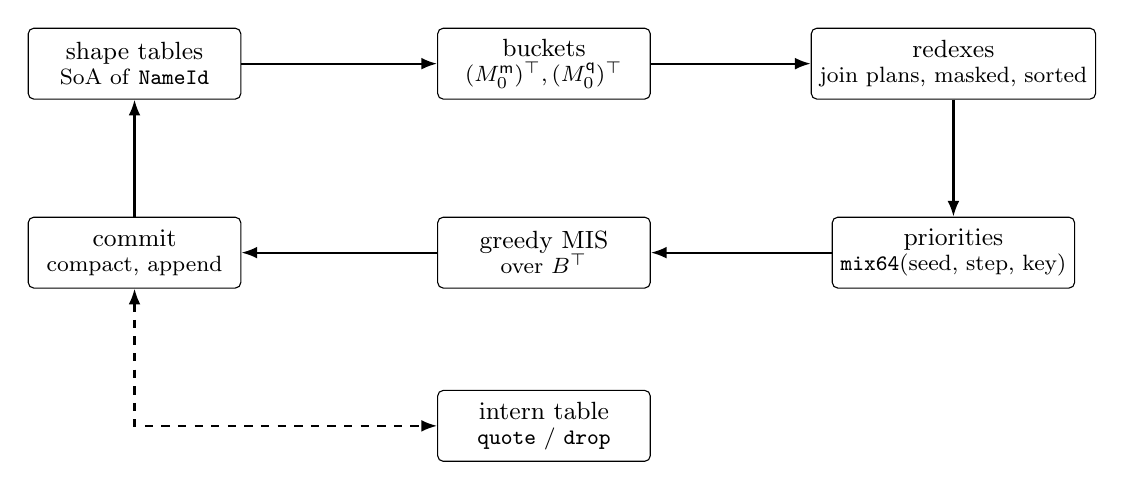
\begin{tikzpicture}[
  box/.style={draw, rounded corners=2pt, align=center, font=\small,
              minimum height=9mm, minimum width=27mm, inner sep=3pt},
  ar/.style={-{Latex[length=2mm]}, thick}]
\node[box] (st)  at (0,0)    {shape tables\\[-2pt] \footnotesize SoA of \code{NameId}};
\node[box] (bk)  at (5.2,0)  {buckets\\[-2pt] \footnotesize $(M^{\mm}_{0})^{\top}, (M^{\qq}_{0})^{\top}$};
\node[box] (rdx) at (10.4,0) {redexes\\[-2pt] \footnotesize join plans, masked, sorted};
\node[box] (pr)  at (10.4,-2.4) {priorities\\[-2pt] \footnotesize \code{mix64}(seed, step, key)};
\node[box] (mis) at (5.2,-2.4)  {greedy MIS\\[-2pt] \footnotesize over $B^{\top}$};
\node[box] (fire) at (0,-2.4)   {commit\\[-2pt] \footnotesize compact, append};
\node[box] (tab) at (5.2,-4.6)  {intern table\\[-2pt] \footnotesize \code{quote} / \code{drop}};
\draw[ar] (st)  -- (bk);
\draw[ar] (bk) -- (rdx);
\draw[ar] (rdx) -- (pr);
\draw[ar] (pr) -- (mis);
\draw[ar] (mis) -- (fire);
\draw[ar] (fire) -- (st);
\draw[{Latex[length=2mm]}-{Latex[length=2mm]},dashed,thick] (fire) |- (tab);
\end{tikzpicture}}
\end{center}

\noindent
This is \cite[Fig.~2]{matnote} with two changes: the conflict product is
replaced by its transpose (Requirement~\ref{req:hyper}), and a priority stage
is made explicit, because it is what the backends must agree on.

\subsection{Backends}

\begin{lstlisting}
pub trait Backend {
    fn find(&mut self, st: &State, plans: &Plans, out: &mut RedexSet);
    fn select(&mut self, r: &RedexSet, prio: &PrioFn, out: &mut Vec<u32>);   // indices into r
    fn commit(&mut self, st: &mut State, it: &mut InternTable, r: &RedexSet,
              sel: &[u32]) -> Result<StepReport, Diag>;
}
pub struct HostSequential;                  // greedy scan; the reference
pub struct HostThreaded { pub cores: u32 }  // std::thread::scope; rounds of Prop. 6.6
\end{lstlisting}

\begin{requirement}[Threaded backend]\label{req:threads}
\code{HostThreaded} \MUST{} use only \code{std::thread::scope}, \MUST{}
partition work by contiguous ranges of consumer rows and of redexes, and
\MUST{} merge results in range order. On \code{wasm32} it \MUST{} fall back to
\code{HostSequential}, reporting \code{cores = 1}. Its output \MUST{} be
bit-identical to \code{HostSequential}'s at every core count
(Requirement~\ref{req:det}).
\end{requirement}

\subsection{The device seam}\label{sec:device}

\begin{requirement}[Device backends live outside the workspace]
\label{req:device}
A device backend necessarily depends on a device API, which the workspace
forbids \cite[Req.~12.3]{combspec}. It \MUST{} therefore be a separate crate
in a separate repository, implementing \code{Backend} against the
\code{.cmat} layout, and \MUST{} be accepted only if its step traces equal
\code{HostSequential}'s under the same seed on the conformance corpus
(Obligation~\ref{obl:devconf}). Its kernels are fixed by this document:
bucketing is a sort by key; each join plan is a segmented expansion over
buckets; masks are elementwise; priorities are \code{mix64} per redex;
selection is the rounds of Proposition~\ref{prop:greedyrounds}; commit is a
stable compaction plus an append by prefix sum; encode is a batched
insert-or-get; decode is a gather from the arena. No work on it \MAY{} begin
before Obligation~\ref{obl:width} is discharged.
\end{requirement}

%======================================================================
\section{Correctness obligations and testing}\label{sec:test}

\begin{obligation}[Round trip]\label{obl:roundtrip}
Requirement~\ref{req:export}: import-export is the identity on encodings and
export-import the identity on markings, for the \Comb{} property generator's
output and for random states over all enabled shapes.
\end{obligation}

\begin{obligation}[Finder agreement]\label{obl:finders}
Requirement~\ref{req:finders}, generalising the reference's
\code{validate}: on at least 10{,}000 random states over all enabled shapes,
two to five names and two to twelve atoms --- the reference's generator,
widened --- the three finders return identical sorted redex sets.
\end{obligation}

\begin{obligation}[Python parity]\label{obl:pyparity}
On the E1--E4 families, the Rust machine \MUST{} reproduce every column of
\code{results.txt} except timing: atoms, parallel steps, rewrites, sequential
steps, maximum width, maximum enumerated redexes, and the ratio. These are
seed-independent for the four families, so the check is exact, and it is a
golden file. They are also laws, and \MUST{} be tested as laws over their
parameters: E1 takes exactly $d$ steps and $kd$ rewrites; E2 one step, $c$
rewrites and $c^{2}$ enumerated; E3 $h+1$ steps and $2^{h+1}-1$ rewrites;
E4 two steps and $2k$ rewrites. On random states, redex sets \MUST{} agree
with the Python reference up to the id bijection, via
Requirement~\ref{req:pyinterop}, as a development tool outside CI.
\end{obligation}

\begin{obligation}[Trace certification]\label{obl:certify}
Every maximal-progress step \MUST{} be certifiable: \code{f1r3comb-check}
linearises it in canonical order and replays each firing with an independent
single-redex rewriter written directly from \cite[Def.~4.6]{combspec} against
\code{Term}s --- not from the rule table --- checking that each is a valid
rewrite and that the final term equals the export of the step's result. This
is \cite[Thm.~8.3]{matnote} tested against a second reading of the rules.
\end{obligation}

\begin{obligation}[Differential against \Comb's machine and \Bell]
\label{obl:diff}
For corpus programs whose observations are resolver-independent (confluent
on encoded observations), the quiescent observation of \Mat{}, of
\code{f1r3comb-run} and of \Bell{} \MUST{} agree, with observation as in
\cite[Obl.~10.4]{combspec}: messages at encodings of source names only. For
the rest, \Mat's final state \MUST{} be certified by
Obligation~\ref{obl:certify}, since the three machines are entitled to
different results.
\end{obligation}

\begin{obligation}[Operator correctness]\label{obl:op}
On random $\ev$-free terms under the exploration budget: \code{successors}
matches the closed formula (Remark in Section~\ref{sec:op}); $T$ is strictly
triangular in the marking order; $T^{\Wt_{0}+1} = 0$; the \code{Bool} closure
equals BFS reachability; every terminal marking of the reach is reached by
some maximal-progress run under some seed in a sample, and every
maximal-progress run's final marking is terminal in the reach.
\end{obligation}

\begin{obligation}[Determinism]\label{obl:det}
The trace, the reports and the \code{.cmat} of the final state \MUST{} be
bit-identical across \code{HostSequential} and \code{HostThreaded} at 1, 2,
7 and 64 cores, and across native and \code{wasm32}, on the whole corpus.
\end{obligation}

\begin{obligation}[Invariants]\label{obl:inv}
Requirement~\ref{req:grading}'s assertions hold on every step of every
corpus run; Requirement~\ref{req:quietjoin} holds for every consumer shape;
the counterexamples of Errata~\ref{err:atomcount}, \ref{err:msgcount} and
\ref{err:symmetric} are regression tests with the corrected expectations.
\end{obligation}

\begin{obligation}[Device conformance]\label{obl:devconf}
A conformance corpus of \code{.cmat} files, seeds and expected step traces
\MUST{} be published from \code{f1r3comb-check} for use by external
backends, and regenerated only by an explicit command.
\end{obligation}

\begin{obligation}[The width of real programs]\label{obl:width}
\cite[Obl.~13.7]{matnote}, unchanged in content: measure the width
distribution of compiled K0 programs with Requirement~\ref{req:widthcmd}. It
needs \Comb{} through its milestone M2. It gates Section~\ref{sec:device} and
nothing else in this document.
\end{obligation}

%======================================================================
\section{Errors and diagnostics}\label{sec:errors}

Diagnostics follow \cite[Req.~11.1]{combspec}: a stable code, a message, no
panic on any input, names rendered by content hash.

\begin{center}
\begin{tabularx}{\linewidth}{@{}ll>{\raggedright\arraybackslash}X@{}}
\toprule
Code & Where & Meaning\\
\midrule
\code{comb-mat-presentation} & any & Built or invoked under
\code{presentation-b} (Decision~\ref{dec:aonly})\\
\code{comb-feature-mismatch} & import & A \code{.cmat} or term with a
different \code{shortcuts} setting; shared with \Comb\\
\code{comb-name-budget} & step & Requirement~\ref{req:budget}; shared with
\Comb\\
\code{comb-mat-hash-collision} & boundary & Requirement~\ref{req:keyhash}\\
\code{comb-mat-overflow} & sparse, op & Checked \code{Nat} arithmetic
overflowed\\
\code{comb-mat-decode} & import & Malformed \code{.cmat}: bad magic,
version, tag, or an id referring forward\\
\code{comb-op-destructor} & op & Exploration of a term that can reach an
$\ev$ row, without a depth bound\\
\code{comb-op-budget} & op & Exploration budget exceeded\\
\code{comb-mat-internal} & any & An invariant assertion failed in a build
that checks it; names the requirement\\
\bottomrule
\end{tabularx}
\end{center}

%======================================================================
\section{Performance, portability, determinism}\label{sec:perf}

\begin{requirement}[Complexity]\label{req:complexity}
Import \MUST{} be linear in the encoding size plus the interning of names.
A step \MUST{} cost $O(n \log n + E + F)$ for $n$ rows, $E$ enumerated
redexes and $F$ produced rows plus arena reads, with $n \log n$ replaceable
by $n$ under radix bucketing; it \MUSTNOT{} depend on the size of the intern
table. Selection \MUST{} be $O(E \log E)$ sequentially (the sort) and
$O(\mathrm{nnz}(B))$ beyond it.
\end{requirement}

\begin{requirement}[Targets]\label{req:targets}
Budget figures for a first implementation, on the reference machine of
\cite[\S11]{k1ndl1ng}, to be re-stated once measured: E1 at $k = 10^{5}$,
$d = 8$ in under one second sequential; import of $10^{5}$ atoms in under
100\,ms; steady-state $10^{7}$ fired redexes per second at 16 cores on
wide terms.
\end{requirement}

\begin{requirement}[Portability]\label{req:port}
As \cite[Req.~12.3]{combspec}: \code{wasm32-unknown-unknown} without
\code{wasm-bindgen}, \code{forbid(unsafe\_code)}, no external dependency.
\code{HashMap} \MAY{} be used only with a fixed-key hasher defined in the
crate, never \code{RandomState}, because iteration order must never be
observable and must never vary.
\end{requirement}

\begin{requirement}[Determinism]\label{req:det}
Given the same term, seed, resolver and configuration, every trace, report
and export \MUST{} be bit-identical across runs, hosts, core counts, and
WebAssembly versus native. No code path \MAY{} iterate a hash map to produce
an ordered result.
\end{requirement}

%======================================================================
\section{What the implementation asks of the papers}\label{sec:paper}

\begin{enumerate}[leftmargin=1.8em]

\item \textbf{Draft~3, Lemma~9.2 and Proposition~9.9}
(Erratum~\ref{err:atomcount}). The lemma is false for $\bl$, $\br$, $\sy$ and
the proposition's bound fails on $\bl(a,b) \mid \mm(a,v) \mid \mm(v,x)$.
Proposed amendment: restate the lemma for the grading $\Wt$, and the bound as
$\Wt(T) \le 2N$. Strong normalisation, and the lattice edge it supports, are
unaffected.

\item \textbf{Matrix note, Theorem~6.1(ii) and Corollary~6.2}. The
nilpotency index is $\Wt(T)+1$, not $N+1$, and the closure needs
$\lceil \log_{2}(\Wt+1) \rceil$ squarings. The grading is the one in
item~1.

\item \textbf{Matrix note, Theorem~6.1(iii)} (Erratum~\ref{err:msgcount}).
Restore draft~3's qualification: the non-increasing quantity is messages plus
stores.

\item \textbf{Matrix note, Proposition~5.3 versus the reference}
(Erratum~\ref{err:symmetric}). The proposition is right and the reference's
enumeration is not; say which count \code{run\_sequential} samples from, since
\cite[Obl.~13.1]{matnote} compares resolvers by their distributions.

\item \textbf{Matrix note, Remark~3.1 and \Comb{} Decision~4.9.} State in
both places that the $\qq$ payload is sorted as a process and represented as
its quotation, and that the shape tag carries the distinction the logic
needs (Decision~\ref{dec:qrow}). As written, a reader of the two documents
together sees a contradiction that is not there.

\item \textbf{\Comb{} v0.2, Requirement~4.7.} Move the rule table to
\code{f1r3comb-term} (Decision~\ref{dec:ruletable}), and give it the fields
\Mat{} reads: premise subjects, datum kind, conclusion template, class.

\item \textbf{\Comb{} v0.2, Requirement~8.3.} Scope the prohibition on
decoding by projection to the \Camp{} machine and to builds where
\code{presentation-b} is reachable, citing Decision~\ref{dec:decode}.

\item \textbf{Draft~3, Remarks~3.10 and~6.7.} State the rules of $\conse$ and
$\consf$ (Decision~\ref{dec:shortcuts}).

\item \textbf{Matrix note, Remark~8.7.} With shared priorities the greedy and
the parallel independent sets coincide (Proposition~\ref{prop:greedyrounds}).
The remark can say so, and P4's exit criterion then follows rather than
having to be engineered.

\item \textbf{Matrix note, Obligation~13.2} is discharged by \Comb's
encoding hash plus in-run structural interning
(Requirement~\ref{req:hashfree}).

\item \textbf{Reference, \code{experiments.py}.} The E4 docstring says each
gadget ``forwards'' the constructed name before opening it; the code builds
$\consm(a,b,c) \mid \mm(a,u) \mid \mm(b,v) \mid \ev(c)$, with no forwarder, and
allocates an unused name $f$. The measurements are right for the code.

\end{enumerate}

%======================================================================
\section{Open questions and deferred work}

\begin{enumerate}[leftmargin=1.8em]
\item \textbf{Resolver fidelity and fairness}
(\cite[Obl.~13.1, Obl.~13.6]{matnote}). \Mat{} makes the resolver a named
parameter and makes all three reproducible, which is what the comparison
needs; the comparison itself is research.
\item \textbf{Contention remedies} (Requirement~\ref{req:contention}). Which
join, and whether priority-ordered lazy enumeration can meet the
identical-step requirement cheaply.
\item \textbf{Contention-set reconciliation} (\cite[Obl.~13.4]{matnote}). The
hypergraph selection of Section~\ref{sec:select} against the contention-set
normalisation of the graded where-clause work. \Mat{}'s selection is fixed by
Definition~\ref{def:step} until that reconciliation says otherwise.
\item \textbf{Garbage} (\cite[Obl.~13.3]{matnote}). Inert rows are counted
(Requirement~\ref{req:reports}); sidelining them from the joins is cheap and
is a v0.2 candidate. Intern-table collection needs reachability from live
rows and is not attempted.
\item \textbf{The history unfolding} (\cite[\S6.1, route (1)]{matnote}), for
triangularity with $\ev$ present.
\item \textbf{Occupancy and nilpotency} (\cite[Obl.~13.5]{matnote}). With the
operator layer in hand, whether the logic's decidable-occupancy requirement
coincides with Erratum~\ref{err:atomcount}'s grading is testable on the
lattice corpus of \cite[Req.~9.3]{combspec}.
\item \textbf{Weights.} A \code{Semiring} instance with per-rule-instance
factors $D_{r}$ \cite[\S12]{matnote}; separate note.
\end{enumerate}

%======================================================================
\section{Delivery}

\begin{center}
\begin{tabularx}{\linewidth}{@{}ll>{\raggedright\arraybackslash}X@{}}
\toprule
M & Deliverable & Done when\\
\midrule
X0 & \code{f1r3comb-mat} & Intern table, shape tables, import, export,
\code{.cmat}, sparse layer; round trip (Obl.~\ref{obl:roundtrip});
key/hash agreement; canonical \code{.cmat} under $\scong$. Needs \Comb{} M0\\
X1 & Finders & Rule table moved to \code{f1r3comb-term}; join plans derived;
\code{Naive}, \code{Product}, \code{Bucketed}; symmetry mask; finder agreement
(Obl.~\ref{obl:finders})\\
X2 & \code{f1r3comb-par}, sequential & Priority, greedy step, commit order,
budgets, reports, traces; Python parity (Obl.~\ref{obl:pyparity}); trace
certification (Obl.~\ref{obl:certify}); invariants (Obl.~\ref{obl:inv})\\
X3 & The width gate & \code{comb-width}; Obligation~\ref{obl:width} run on the
\Comb{} corpus and reported. Needs \Comb{} M2. \textbf{Gate} on the device
seam\\
X4 & Threaded host & \code{HostThreaded}; determinism across cores and
\code{wasm32} (Obl.~\ref{obl:det}); differential tests (Obl.~\ref{obl:diff});
targets re-stated\\
X5 & \code{f1r3comb-op} & Successors, exploration, $T$, closure, \code{pre};
operator correctness (Obl.~\ref{obl:op}); \code{comb-op}\\
X6 & Device conformance & Corpus and expected traces published
(Obl.~\ref{obl:devconf}); external backend work only if X3 says so\\
\bottomrule
\end{tabularx}
\end{center}

\noindent
X0--X2 are the representation and a correct machine, independently useful:
they give \cite{matnote} a checked port of its reference, and they give
\Comb{} a second, differently resolved machine to test against. X3 is the
single number on which the accelerator enterprise stands or falls
\cite[Princ.~10.4]{matnote}. X5 is independent of X3 and X4, and its natural
consumer is the logic.

%======================================================================
\appendix
\section{Correspondence with the reference implementation}\label{app:corr}

\begin{center}\small
\begin{tabularx}{\linewidth}{@{}l>{\raggedright\arraybackslash}X@{}}
\toprule
\code{rhocombmat.py} & \Mat\\
\midrule
\code{ARITY}, \code{SHAPES} & \code{Shape}, arities from the rule table;
\code{cons} is \code{Shape::Cons} ($\cons_{\mid}$)\\
\code{NameTable.quote} / \code{drop} & \code{InternTable::quote} /
\code{drop}, keyed structurally (Def.~\ref{def:skey})\\
\code{State.occ} (dict of occurrence ids) & Shape tables; occurrence identity
is the row ref, stable within a step (Req.~\ref{req:insertorder})\\
\code{incidence} & Implicit (Def.~\ref{def:inc});
\code{Csr::from\_column} for the \code{Product} finder\\
\code{redexes\_matrix} & \code{Product} finder, plus the symmetry mask\\
\code{redexes\_naive} & \code{Naive} finder\\
\code{BINARY\_M}, the $\mathsf{quote}$ join, the 3- and 4-premise
joins & Derived join plans (Def.~\ref{def:plan})\\
\code{conflict\_graph} ($BB^{\top}$) & Reference only; production uses
$B^{\top}$ (Req.~\ref{req:hyper})\\
\code{mis} (shuffled greedy) & Greedy by \code{mix64} priority
(Def.~\ref{def:step}); identical to the rounds algorithm\\
\code{fire} & \code{commit}, with fixed effect order\\
\code{run\_parallel} & \code{Resolver::MaximalProgress}\\
\code{run\_sequential} & \code{Resolver::SingleUniform}\\
\code{experiments.fan}, \code{contended}, \code{dup\_tree},
\code{construct\_then\_eval} & \code{f1r3comb-check} families E1--E4, golden
against \code{results.txt}\\
\code{validate} & Obligation~\ref{obl:finders}\\
q payload held as a name & Decision~\ref{dec:qrow}\\
\bottomrule
\end{tabularx}
\end{center}

%======================================================================
\begin{thebibliography}{99}

\bibitem{matnote} L.\,G. Meredith.
\emph{Rho combinators as sparse linear algebra: a classical route from
reflective concurrency to data-parallel execution.} Version~1,
\code{publications/rho-combinators/rhocomb-matrix}, with
\code{rhocombmat.py}, \code{experiments.py} and \code{results.txt},
September 2026.

\bibitem{combspec} F1R3FLY.io.
\emph{F1R3Comb: a compiler from kernel rho to the name-free rho combinators,
and a machine that runs the result.} Specification v0.2,
\code{publications/rho-combinators/f1r3comb-spec-v02}, September 2026.

\bibitem{draft3} L.\,G. Meredith and M. Stay.
\emph{Name-free combinators for the rho calculus: a repair, a linear encoding,
and the one operation that was missing.} Draft~3,
\code{publications/rho-combinators}, September 2026.

\bibitem{logic} F1R3FLY.io.
\emph{A spatial-behavioural logic for the rho combinators.} Draft~2,
\code{publications/rho-combinators/rhocomb-logic}, September 2026.

\bibitem{k1ndl1ng} F1R3FLY.io.
\emph{K1ndl1ng: a parser and normaliser for kernel rholang.}
\code{publications/campf1r3/k1ndl1ng-spec}, 2026.

\bibitem{campf1r3} F1R3FLY.io.
\emph{CampF1R3: an in-memory tuple space.}
\code{publications/campf1r3/campf1r3-spec}, 2026.

\bibitem{bfs} G.\,E. Blelloch, J.\,T. Fineman and J. Shun.
Greedy sequential maximal independent set and matching are parallel on
average. \emph{SPAA}, 2012.

\bibitem{luby} M. Luby.
A simple parallel algorithm for the maximal independent set problem.
\emph{SIAM Journal on Computing}, 1986.

\bibitem{gustavson} F.\,G. Gustavson.
Two fast algorithms for sparse matrices: multiplication and permuted
transposition. \emph{ACM Transactions on Mathematical Software}, 1978.

\bibitem{splitmix} G.\,L. Steele, D. Lea and C.\,H. Flood.
Fast splittable pseudorandom number generators. \emph{OOPSLA}, 2014.

\bibitem{ngo} H.\,Q. Ngo, E. Porat, C. R\'e and A. Rudra.
Worst-case optimal join algorithms. \emph{Journal of the ACM}, 2018.

\bibitem{graphblas} J. Kepner and J. Gilbert (eds.).
\emph{Graph Algorithms in the Language of Linear Algebra}. SIAM, 2011.

\bibitem{baezbiamonte} J. Baez and J. Biamonte.
\emph{Quantum Techniques for Stochastic Mechanics}. World Scientific, 2018.

\end{thebibliography}

\end{document}
